\documentclass[12pt, a4paper]{book}
\usepackage[T1]{fontenc}
\usepackage[utf8]{inputenc}
\usepackage[charter, cal=cmcal]{mathdesign}
\usepackage[scaled=0.92]{helvet}
\usepackage{geometry}
\geometry{a4paper, top=30mm, bottom=30mm, inner=32mm, outer=25mm}
\usepackage{amsmath, amssymb}
\usepackage[version=4]{mhchem}
\usepackage[dvipsnames,svgnames,table]{xcolor}
\usepackage{tikz}
\usetikzlibrary{arrows.meta, positioning, calc, backgrounds}
\usepackage{pgfplots}
\pgfplotsset{compat=1.18}
\usepackage{tcolorbox}
\tcbuselibrary{skins, breakable}
\usepackage{titlesec}
\usepackage{fancyhdr}
\usepackage{enumitem}
\usepackage{booktabs}
\usepackage{array}
\usepackage{parskip}
\usepackage{siunitx}
\usepackage{multicol}
\usepackage[colorlinks=true, linkcolor=BrickRed, urlcolor=NavyBlue]{hyperref}

\definecolor{JourneyColor}{HTML}{1A5276}
\definecolor{ModuleColor}{HTML}{2E86C1}
\definecolor{PuzzleColor}{HTML}{145A32}
\definecolor{DiscoveryColor}{HTML}{B7950B}
\definecolor{WarningColor}{HTML}{C0392B}
\definecolor{ProblemColor}{HTML}{4A235A}
\definecolor{ReflectColor}{HTML}{117A65}
\definecolor{HistoryColor}{HTML}{6E2F1A}
\definecolor{HBondColor}{HTML}{7D3C98}
\definecolor{LDFColor}{HTML}{1E8449}
\definecolor{DipoleColor}{HTML}{1A5276}

\newtcolorbox{puzzlebox}[1][]{enhanced,breakable,
  colback=PuzzleColor!6,colframe=PuzzleColor,fonttitle=\bfseries\sffamily,
  title={The Puzzle},attach boxed title to top left={yshift=-2mm,xshift=6mm},
  boxed title style={colback=PuzzleColor},borderline west={3pt}{0pt}{PuzzleColor},#1}
\newtcolorbox{discoverybox}[1][]{enhanced,breakable,
  colback=DiscoveryColor!8,colframe=DiscoveryColor,fonttitle=\bfseries\sffamily,
  title={Discovery},attach boxed title to top left={yshift=-2mm,xshift=6mm},
  boxed title style={colback=DiscoveryColor},borderline west={3pt}{0pt}{DiscoveryColor},#1}
\newtcolorbox{problembox}[1][]{enhanced,breakable,
  colback=ProblemColor!5,colframe=ProblemColor,fonttitle=\bfseries\sffamily,
  title={Problems},attach boxed title to top left={yshift=-2mm,xshift=6mm},
  boxed title style={colback=ProblemColor},borderline west={3pt}{0pt}{ProblemColor},#1}
\newtcolorbox{deepbox}[1][]{enhanced,breakable,
  colback=JourneyColor!5,colframe=JourneyColor,fonttitle=\bfseries\sffamily,
  title={Deep Problems},attach boxed title to top left={yshift=-2mm,xshift=6mm},
  boxed title style={colback=JourneyColor},borderline west={4pt}{0pt}{JourneyColor},#1}
\newtcolorbox{reflectionbox}[1][]{enhanced,breakable,
  colback=ReflectColor!6,colframe=ReflectColor,fonttitle=\bfseries\sffamily,
  title={Reflection},attach boxed title to top left={yshift=-2mm,xshift=6mm},
  boxed title style={colback=ReflectColor},borderline west={3pt}{0pt}{ReflectColor},#1}
\newtcolorbox{namedconcept}[2][]{enhanced,
  colback=ModuleColor!6,colframe=ModuleColor,fonttitle=\bfseries\sffamily\large,
  title={#2},attach boxed title to top left={yshift=-2mm,xshift=6mm},
  boxed title style={colback=ModuleColor},#1}

\titleformat{\chapter}[display]
  {\normalfont\sffamily\huge\bfseries\color{JourneyColor}}
  {\textcolor{JourneyColor!60}{\chaptertitlename\ \thechapter}}{10pt}{\Huge}
  [\vspace{2pt}\textcolor{JourneyColor}{\titlerule[1.5pt]}]
\titleformat{\section}{\normalfont\sffamily\Large\bfseries\color{ModuleColor}}
  {\thesection}{1em}{}[\textcolor{ModuleColor!40}{\titlerule[0.6pt]}]
\titleformat{\subsection}{\normalfont\sffamily\large\bfseries\color{JourneyColor!80}}
  {\thesubsection}{1em}{}
\pagestyle{fancy}\fancyhf{}
\fancyhead[LE]{\small\sffamily\textcolor{JourneyColor}{\leftmark}}
\fancyhead[RO]{\small\sffamily\textcolor{ModuleColor}{\rightmark}}
\fancyfoot[C]{\small\thepage}
\renewcommand{\headrulewidth}{0.4pt}
\newcommand{\newterm}[1]{\textit{\textcolor{DiscoveryColor}{#1}}}

\begin{document}
\setcounter{chapter}{3}
\chapter[Journey 4 --- The Bond]{Journey Four\\[8pt]
  \textcolor{ModuleColor}{\large The Bond: Why Atoms Stick Together}}
\setcounter{section}{4}

\section{Module 4.5 --- Intermolecular Forces: Between Molecules}

\subsection*{Motivation}

Covalent bonds hold atoms together within a molecule.
Intermolecular forces hold molecules together in liquids and solids.

These forces are 10--100 times weaker than covalent bonds,
yet they determine nearly everything we experience:
whether a substance is a gas or a liquid at room temperature,
how substances mix, the viscosity of oils, the surface tension
of water, the structure of DNA, the folding of proteins.

This module builds the hierarchy of intermolecular forces
from their quantum mechanical origins,
and uses them to explain macroscopic properties.

\subsection{The Hierarchy of Intermolecular Forces}

\begin{center}
\small
\begin{tabular}{llll}
\toprule
Force & Origin & Strength (kJ/mol) & Molecules affected \\
\midrule
Ion-dipole      & charge + dipole & 40--600 & ions in polar solvents \\
Hydrogen bond   & N/O/F--H$\cdots$N/O/F & 10--40  & \ce{H2O}, \ce{NH3}, DNA \\
Dipole-dipole   & two permanent dipoles & 1--10   & polar molecules \\
London dispersion & induced dipoles & 0.1--40 & all molecules \\
\bottomrule
\end{tabular}
\end{center}

\vspace{0.5em}

All intermolecular forces are ultimately electrostatic.
The differences arise from whether the charges are permanent
or instantaneous, fixed or fluctuating.

\subsection{London Dispersion Forces: The Universal Attraction}

\newterm{London dispersion forces} (also called van der Waals
forces or induced dipole--induced dipole forces) act between
\emph{all} molecules, including noble gases and nonpolar molecules.

\begin{namedconcept}{Origin of London Forces}
At any instant, the electron cloud of a molecule has an
asymmetric distribution --- a temporary dipole.
This temporary dipole induces a dipole in a neighbouring molecule.
The two instantaneous dipoles attract each other.

The time-averaged dipole is zero (nonpolar molecule),
but the time-averaged \emph{interaction energy} is negative
(attractive) because favourable alignments are
energetically preferred.

Magnitude scales with:
\begin{itemize}[nosep, leftmargin=2em]
  \item \textbf{Polarisability} $\alpha$: how easily the electron
        cloud distorts. Larger, more diffuse electron clouds
        are more polarisable. Polarisability increases
        down a group (more electrons, farther from nucleus).
  \item \textbf{Distance}: $V_\text{LDF} \propto -1/r^6$
        (very short range).
  \item \textbf{Surface area}: more contact area between molecules
        means more interaction.
\end{itemize}
\end{namedconcept}

\begin{center}
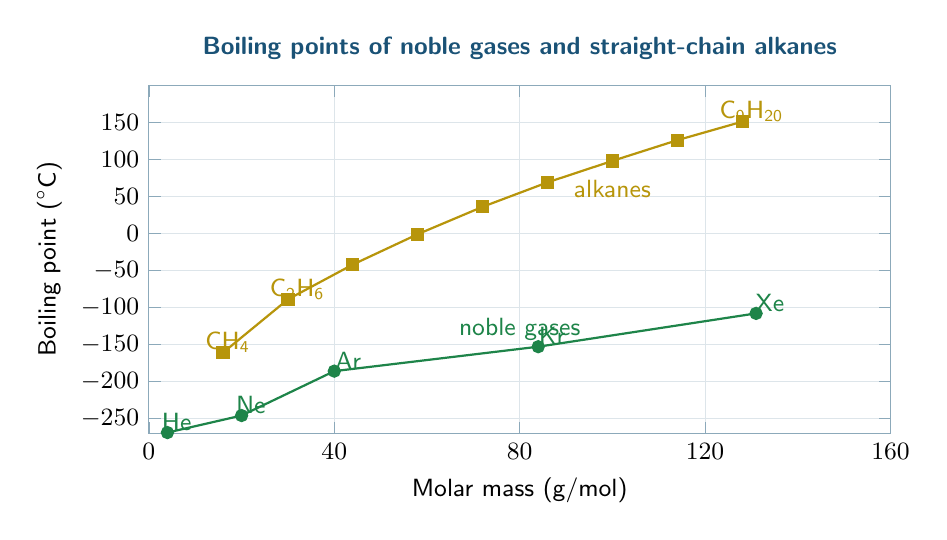
\begin{tikzpicture}[every node/.style={font=\sffamily\small}]
  \begin{axis}[
    width=11cm, height=6cm,
    xlabel={Molar mass (g/mol)},
    ylabel={Boiling point ($^\circ$C)},
    xmin=0, xmax=160,
    ymin=-270, ymax=200,
    xtick={0,40,80,120,160},
    ytick={-250,-200,-150,-100,-50,0,50,100,150},
    grid=major,
    grid style={line width=0.3pt, draw=JourneyColor!15},
    axis line style={color=JourneyColor!50},
    tick style={color=JourneyColor!50},
    title style={font=\sffamily\small\bfseries, color=JourneyColor},
    title={Boiling points of noble gases and straight-chain alkanes},
    label style={font=\sffamily\small}
  ]
    % Noble gases
    \addplot[thick, color=LDFColor, mark=*, mark size=2pt]
      coordinates {(4,-269)(20,-246)(40,-186)(84,-153)(131,-108)};
    \node[font=\sffamily\small, text=LDFColor]
      at (axis cs:80,-130) {noble gases};

    % Alkanes
    \addplot[thick, color=DiscoveryColor, mark=square*, mark size=2pt]
      coordinates {(16,-161)(30,-89)(44,-42)(58,-1)(72,36)(86,69)(100,98)(114,126)(128,151)};
    \node[font=\sffamily\small, text=DiscoveryColor]
      at (axis cs:100,60) {alkanes};

    % Labels for noble gases
    \node[font=\sffamily\small, text=LDFColor] at (axis cs:6,-255) {He};
    \node[font=\sffamily\small, text=LDFColor] at (axis cs:22,-232) {Ne};
    \node[font=\sffamily\small, text=LDFColor] at (axis cs:43,-172) {Ar};
    \node[font=\sffamily\small, text=LDFColor] at (axis cs:87,-139) {Kr};
    \node[font=\sffamily\small, text=LDFColor] at (axis cs:134,-94) {Xe};

    % Labels for selected alkanes
    \node[font=\sffamily\small, text=DiscoveryColor] at (axis cs:17,-147) {\ce{CH4}};
    \node[font=\sffamily\small, text=DiscoveryColor] at (axis cs:32,-75) {\ce{C2H6}};
    \node[font=\sffamily\small, text=DiscoveryColor] at (axis cs:130,165) {\ce{C9H20}};
  \end{axis}
\end{tikzpicture}
\end{center}

\vspace{0.3em}

Both noble gases and alkanes are nonpolar ---
only London forces operate.
The boiling point increases with molar mass in both series
because larger molecules have more electrons and greater
polarisability.

\subsection{Hydrogen Bonds: The Special Case}

Hydrogen bonds are \emph{not} covalent bonds.
They are electrostatic attractions between a hydrogen atom
covalently bonded to a highly electronegative atom
(N, O, or F) and a lone pair on another electronegative atom.

\[
  \text{X--H} \cdots \text{Y}
  \qquad
  \text{where X, Y} \in \{\text{N, O, F}\}
\]

\begin{namedconcept}{Why Hydrogen Bonds Are Special}
Hydrogen is unique: it has no inner electrons to shield
its nucleus.
When bonded to F, O, or N, its electron density is strongly
pulled away, leaving a nearly ``bare proton'' that can
approach the lone pair of another electronegative atom
unusually closely.

The H-bond energy (10--40 kJ/mol) is much larger than
typical London forces between comparable molecules,
but much weaker than covalent bonds ($>$ 150 kJ/mol).

H-bonds are:
\begin{itemize}[nosep, leftmargin=2em]
  \item \textbf{Directional}: the X--H$\cdots$Y angle is
        typically $150$--$180^\circ$.
  \item \textbf{Cooperative}: one H-bond facilitates the
        next (important in water and protein $\alpha$-helices).
  \item \textbf{Dynamic}: constantly breaking and reforming
        in liquid water (lifetime $\sim 1$ ps).
\end{itemize}
\end{namedconcept}

\begin{center}
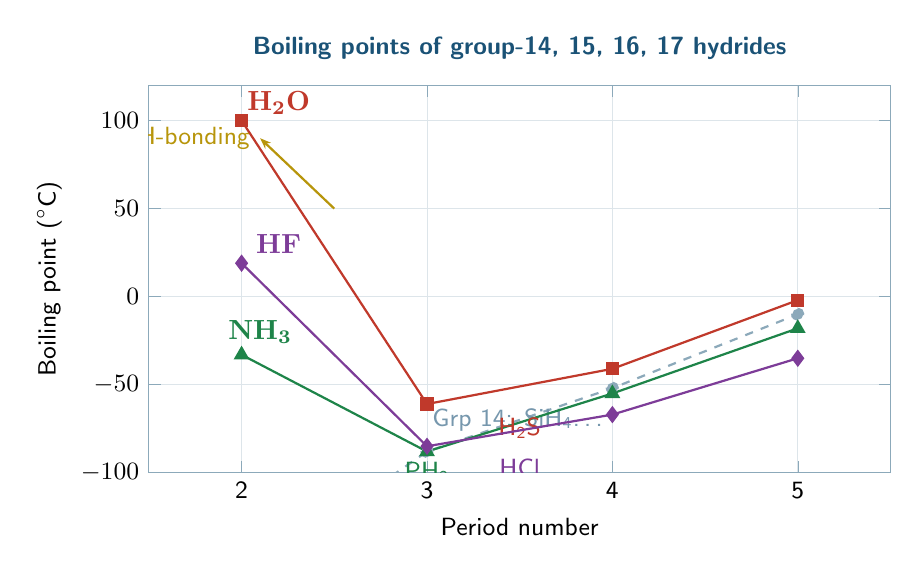
\begin{tikzpicture}[every node/.style={font=\sffamily\small}]
  \begin{axis}[
    width=11cm, height=6.5cm,
    xlabel={Period number},
    ylabel={Boiling point ($^\circ$C)},
    xmin=1.5, xmax=5.5,
    ymin=-100, ymax=120,
    xtick={2,3,4,5},
    xticklabels={2,3,4,5},
    ytick={-100,-50,0,50,100},
    grid=major,
    grid style={line width=0.3pt, draw=JourneyColor!15},
    axis line style={color=JourneyColor!50},
    tick style={color=JourneyColor!50},
    title style={font=\sffamily\small\bfseries, color=JourneyColor},
    title={Boiling points of group-14, 15, 16, 17 hydrides},
    label style={font=\sffamily\small}
  ]
    % Group 14 (no H-bond, reference)
    \addplot[thick, color=JourneyColor!50, mark=*, mark size=2pt, dashed]
      coordinates {(2,-161)(3,-88)(4,-52)(5,-10)};
    \node[font=\sffamily\small, text=JourneyColor!60]
      at (axis cs:3.5,-70) {Grp 14: \ce{SiH4}\ldots};

    % Group 15
    \addplot[thick, color=LDFColor, mark=triangle*, mark size=2.5pt]
      coordinates {(2,-33)(3,-88)(4,-55)(5,-18)};
    \node[font=\sffamily\small, text=LDFColor]
      at (axis cs:3,-100) {\ce{PH3}};
    \node[font=\sffamily\small, text=LDFColor, font=\bfseries]
      at (axis cs:2.1,-20) {\ce{NH3}};

    % Group 16
    \addplot[thick, color=WarningColor, mark=square*, mark size=2pt]
      coordinates {(2,100)(3,-61)(4,-41)(5,-2)};
    \node[font=\sffamily\small, text=WarningColor, font=\bfseries]
      at (axis cs:2.2,110) {\ce{H2O}};
    \node[font=\sffamily\small, text=WarningColor]
      at (axis cs:3.5,-75) {\ce{H2S}};

    % Group 17
    \addplot[thick, color=HBondColor, mark=diamond*, mark size=2.5pt]
      coordinates {(2,19)(3,-85)(4,-67)(5,-35)};
    \node[font=\sffamily\small, text=HBondColor, font=\bfseries]
      at (axis cs:2.2,30) {HF};
    \node[font=\sffamily\small, text=HBondColor]
      at (axis cs:3.5,-97) {HCl};

    % Anomaly annotation
    \draw[-{Stealth[length=4pt]}, thick, DiscoveryColor]
      (axis cs:2.5,50) -- (axis cs:2.1,90)
      node[left, font=\sffamily\small, text=DiscoveryColor]
        {Anomalously high: H-bonding};
  \end{axis}
\end{tikzpicture}
\end{center}

\vspace{0.3em}

\ce{H2O}, \ce{HF}, and \ce{NH3} are the three anomalies ---
all far above the trend established by their heavier
group members (which have only London forces and dipole-dipole).
The anomaly is H-bonding.

\subsection{Consequences of H-bonding in Water}

Water's extraordinary properties trace to its network
of hydrogen bonds:

\begin{itemize}[nosep, leftmargin=2em]
  \item \textbf{High boiling point} (b.p. $100^\circ$C vs expected
        $\sim -80^\circ$C from the period-3/4/5 trend).
  \item \textbf{High surface tension}: the strong H-bond network
        at the surface resists disruption.
  \item \textbf{High heat capacity}: breaking and reforming
        H-bonds absorbs energy without raising temperature.
  \item \textbf{Ice less dense than liquid water}: in ice,
        each water molecule forms 4 H-bonds in a fixed
        tetrahedral lattice --- more open than liquid water.
        Ice floats. This is essential for aquatic life in cold climates.
  \item \textbf{Excellent solvent for polar/ionic compounds}:
        strong hydration energy from H-bonding and ion-dipole.
\end{itemize}

\subsection{The van der Waals Equation: Intermolecular Forces and Real Gases}

Ideal gas law: $PV = nRT$.
This assumes no intermolecular forces and no molecular volume.
Real gases deviate, especially at high pressure and low temperature.

Van der Waals (1873) corrected both:
\[
  \left(P + \frac{an^2}{V^2}\right)(V - nb) = nRT
\]
where:
\begin{itemize}[nosep, leftmargin=2em]
  \item $a$ corrects for intermolecular attraction:
        molecules attract each other, reducing the pressure
        they exert on the walls.
  \item $b$ corrects for molecular volume:
        the volume available to the gas is reduced
        by the space occupied by the molecules themselves.
\end{itemize}

\begin{center}
\small
\begin{tabular}{lcc}
\toprule
Gas & $a$ (L$^2$ atm/mol$^2$) & $b$ (L/mol) \\
\midrule
\ce{He}    & 0.034 & 0.024 \\
\ce{H2}    & 0.244 & 0.027 \\
\ce{N2}    & 1.39  & 0.039 \\
\ce{CO2}   & 3.59  & 0.043 \\
\ce{H2O}   & 5.46  & 0.031 \\
\ce{C6H6}  & 18.24 & 0.115 \\
\bottomrule
\end{tabular}
\end{center}

Water has a large $a$ (strong attractions, H-bonding)
but relatively small $b$ (compact molecule).
Benzene has enormous $a$ (large, polarisable, strong LDF)
and large $b$ (physically big molecule).

\begin{problembox}
\begin{enumerate}[label=\textbf{\arabic*.}]
  \item \textbf{Explaining boiling point trends.}

    Arrange each set in order of increasing boiling point
    and explain the dominant intermolecular force for each:
    \begin{enumerate}[label=(\alph*)]
      \item \ce{CH4}, \ce{CF4}, \ce{CCl4}, \ce{CBr4}, \ce{CI4}
      \item \ce{HF}, \ce{HCl}, \ce{HBr}, \ce{HI}
            (Note: HF has the smallest molar mass but the
            highest boiling point in this series. Explain.)
      \item \ce{CH3OH} (methanol), \ce{CH3CH2OH} (ethanol),
            \ce{CH3OCH3} (dimethyl ether)
            (all \ce{C2} compounds with similar molar mass;
            methanol and ethanol can H-bond, ether cannot)
    \end{enumerate}

  \item \textbf{Hydrogen bonding in biology.}

    DNA's double helix is held together by H-bonds between
    complementary base pairs:
    A--T pairs have 2 H-bonds; G--C pairs have 3 H-bonds.
    \begin{enumerate}[label=(\alph*)]
      \item A DNA duplex has 500 base pairs with 60\% G--C
            content.
            Estimate the total number of H-bonds.
      \item The average H-bond energy is $\sim 20$ kJ/mol.
            Estimate the total stabilisation energy from
            H-bonding alone.
      \item The two strands can be separated (``melted'')
            by heating.
            A G--C-rich sequence has a higher melting temperature.
            Explain why, and why this matters for PCR
            (polymerase chain reaction) primer design.
      \item Individual H-bonds have energy $\sim 20$ kJ/mol ---
            roughly 8 $k_BT$ at room temperature ($k_BT \approx 2.5$ kJ/mol).
            Yet DNA remains intact at body temperature.
            Explain: is it the strength of individual H-bonds
            or their number that matters?
    \end{enumerate}

  \item \textbf{Van der Waals equation.}

    A sample of \ce{CO2} ($n = 1.00$ mol) is held in a
    container of $V = 0.500$ L at $T = 300$ K.
    \begin{enumerate}[label=(\alph*)]
      \item Calculate the pressure using the ideal gas law.
      \item Calculate the pressure using the van der Waals
            equation ($a = 3.59$ L$^2$ atm/mol$^2$,
            $b = 0.043$ L/mol).
      \item Which correction is more important at these
            conditions: the $a$ term (attractions) or the
            $b$ term (volume)?
      \item At very high pressures ($V \approx nb$), the
            pressure predicted by van der Waals is
            \emph{higher} than ideal.
            Why? Which term dominates?
    \end{enumerate}
\end{enumerate}
\end{problembox}

\subsection*{Deep Problems}

\begin{deepbox}
\begin{enumerate}[label=\textbf{D\arabic*.}]

  \item \textbf{Gecko adhesion and van der Waals forces.}

    Geckos can walk on smooth vertical surfaces.
    The mechanism: millions of microscopic hair-like setae
    on their feet (each $\sim 100\ \mu$m long, $\sim 5\ \mu$m wide),
    each tipped with even finer ``spatulae'' ($\sim 200$ nm).

    The adhesion is due entirely to London dispersion forces
    between the spatulae and the surface.

    \begin{enumerate}[label=(\alph*)]
      \item A single spatula contacts $\sim 0.1\ \mu$m$^2$ of surface.
            The LDF adhesion energy per unit area for gecko
            setae is estimated as $\sim 0.1\ \text{J/m}^2$.
            Estimate the adhesion force of a single spatula.
      \item A gecko has $\sim 6.5 \times 10^6$ spatulae.
            If all engage simultaneously, what is the total
            maximum adhesion force?
            Compare to the weight of a typical gecko
            ($\sim 70$ g).
      \item Real geckos achieve $\sim 20 \times$ their own weight
            in adhesion.
            The efficiency (fraction of spatulae engaged)
            is much less than 100\%.
            Estimate the fraction from your calculation.
      \item Gecko-inspired synthetic adhesives have been made
            from aligned carbon nanotube arrays.
            What property of CNTs makes them good analogues
            of gecko setae for LDF adhesion?
    \end{enumerate}

  \item \textbf{Why proteins fold.}

    Proteins are chains of amino acids.
    Some amino acids have nonpolar side chains (hydrophobic);
    others have polar or charged side chains (hydrophilic).
    In water, proteins fold so that hydrophobic residues
    are buried inside and hydrophilic ones face the solvent.

    \begin{enumerate}[label=(\alph*)]
      \item Explain the \newterm{hydrophobic effect} in terms
            of entropy.
            When a nonpolar molecule is in water, water
            molecules form ordered ``cages'' around it,
            losing entropy.
            What thermodynamic principle drives the
            nonpolar residues to cluster together?
      \item The hydrophobic effect accounts for $\sim 4$ kJ/mol
            per CH$_2$ group transferred from water to a
            nonpolar environment.
            A protein buries 50 hydrophobic CH$_2$ groups.
            Estimate the contribution to folding stability.
      \item Proteins unfold (denature) when heated.
            Is denaturation enthalpy-driven or entropy-driven?
            (Hint: the unfolded state has more conformational
            entropy; the hydrophobic effect is entropy-driven
            and weakens at high temperature.)
      \item Urea (a small molecule that can H-bond) unfolds
            proteins at high concentration by competing with
            intramolecular H-bonds.
            Explain the mechanism and why urea must be
            present at molar concentrations (6--8 M) rather
            than just millimolar.
    \end{enumerate}

\end{enumerate}
\end{deepbox}

\subsection*{Reflection}

\begin{reflectionbox}
\begin{enumerate}[label=\textbf{R\arabic*.}]
  \item London dispersion forces are due to instantaneous
    dipoles caused by electron fluctuations.
    \textbf{Is it strange that a ``force'' arises from
    something that, when averaged over time, equals zero?}
    What other physical phenomena arise from fluctuations
    that average to zero?

  \item The fact that ice floats is essential for aquatic life:
    a lake freezes from the top down, preserving liquid water
    below.
    \textbf{Is it coincidental that water has these anomalous
    properties, or would any molecule that can hydrogen-bond
    have similar properties?}
    What would happen to life on Earth if water's density
    maximum were above $0^\circ$C?

  \item Protein folding is driven by the hydrophobic effect,
    which is \emph{entropy-driven} (water gains entropy when
    nonpolar groups cluster).
    \textbf{In what sense is the shape of every protein in
    your body a consequence of thermodynamics rather than
    chemistry?}
    Is there a difference?
\end{enumerate}
\end{reflectionbox}

\vspace{1.5em}
\begin{center}
\begin{tcolorbox}[enhanced, colback=DiscoveryColor!8, colframe=DiscoveryColor,
  width=0.88\textwidth, arc=3pt]
\centering\sffamily\small
\textbf{What we invented in this module.}\\[4pt]
All molecules attract each other via London dispersion forces
--- instantaneous dipole fluctuations that scale with
polarisability and surface area.
Polar molecules additionally attract via dipole-dipole forces.
Molecules containing N--H, O--H, or F--H bonds form
hydrogen bonds: strong, directional, and crucial for life.
These forces explain every macroscopic property not
determined by intramolecular chemistry: boiling points,
viscosity, surface tension, solubility, protein folding, DNA structure.
The extraordinary properties of water --- the universal solvent,
the expanding solid, the liquid with anomalously high boiling
point --- all trace to its four hydrogen bonds per molecule.
\end{tcolorbox}
\end{center}

\vspace{2em}
\noindent\textcolor{JourneyColor!40}{\rule{\textwidth}{0.6pt}}
\begin{center}\textit{\sffamily\small
Module 4.5 complete. Continue to Module 4.6:\\
\textbf{Journey 4 Synthesis: The Bonding Continuum}.}
\end{center}
\end{document}